%File: anonymous-submission-latex-2026.tex
\documentclass[letterpaper]{article} % DO NOT CHANGE THIS
\usepackage{aaai2026}  % DO NOT CHANGE THIS
\usepackage{times}  % DO NOT CHANGE THIS
\usepackage{helvet}  % DO NOT CHANGE THIS
\usepackage{courier}  % DO NOT CHANGE THIS
\usepackage[hyphens]{url}  % DO NOT CHANGE THIS
\usepackage{graphicx} % DO NOT CHANGE THIS
\urlstyle{rm} % DO NOT CHANGE THIS
\def\UrlFont{\rm}  % DO NOT CHANGE THIS
\usepackage{natbib}  % DO NOT CHANGE THIS AND DO NOT ADD ANY OPTIONS TO IT
\usepackage{caption} % DO NOT CHANGE THIS AND DO NOT ADD ANY OPTIONS TO IT
\frenchspacing  % DO NOT CHANGE THIS
\setlength{\pdfpagewidth}{8.5in} % DO NOT CHANGE THIS
\setlength{\pdfpageheight}{11in} % DO NOT CHANGE THIS
% \usepackage{courier} % duplicate removed
\usepackage{amsfonts}
\usepackage{tabularx}
\usepackage{multirow}
\usepackage{booktabs}
\usepackage{amsmath}
%
% These are recommended to typeset algorithms but not required. See the subsubsection on algorithms. Remove them if you don't have algorithms in your paper.
\usepackage{algorithm}
\usepackage{algorithmic}
\usepackage{enumitem}
%
% These are are recommended to typeset listings but not required. See the subsubsection on listing. Remove this block if you don't have listings in your paper.
\usepackage{newfloat}
\usepackage{listings}
\DeclareCaptionStyle{ruled}{labelfont=normalfont,labelsep=colon,strut=off} % DO NOT CHANGE THIS
\lstset{%
	basicstyle={\footnotesize\ttfamily},% footnotesize acceptable for monospace
	numbers=left,numberstyle=\footnotesize,xleftmargin=2em,% show line numbers, remove this entire line if you don't want the numbers.
	aboveskip=0pt,belowskip=0pt,%
	showstringspaces=false,tabsize=2,breaklines=true}
\floatstyle{ruled}
\newfloat{listing}{tb}{lst}{}
\floatname{listing}{Listing}
%
% Keep the \pdfinfo as shown here. There's no need
% for you to add the /Title and /Author tags.
\pdfinfo{
/TemplateVersion (2026.1)
}



\setcounter{secnumdepth}{0} %May be changed to 1 or 2 if section numbers are desired.

% The file aaai2026.sty is the style file for AAAI Press
% proceedings, working notes, and technical reports.
%

% Title

% Your title must be in mixed case, not sentence case.
% That means all verbs (including short verbs like be, is, using,and go),
% nouns, adverbs, adjectives should be capitalized, including both words in hyphenated terms, while
% articles, conjunctions, and prepositions are lower case unless they
% directly follow a colon or long dash
\title{Mind the Gap: Predicting, Explaining and Reducing Time‑to‑First‑Comment (Reply Gap) in Online Mental‑Health Communities}

%%\title{The Anatomy of a Choice: Expertise, Trust, and Decision Patterns in Human-AI Co-Creation}
% (Removed example \author and \affiliations from template)

% Camera-ready authors and affiliations
\author{
    Guangrui Fan\thanks{Corresponding author. Email: fgr@tyust.edu.cn}\equalcontrib\textsuperscript{\rm 1},
    Dandan Liu\equalcontrib\textsuperscript{\rm 2},
    Lihu Pan\textsuperscript{\rm 1}
}
\affiliations{
    \textsuperscript{\rm 1}School of Computer Science, Taiyuan University of Science and Technology, Taiyuan, China\\
    \textsuperscript{\rm 2}Department of Media and Communication Studies, Universiti Malaya, Kuala Lumpur, Malaysia\\
    fgr@tyust.edu.cn, s2134717@siswa.um.edu.my, panlh@tyust.edu.cn
}


% (bibentry removed for camera-ready compliance)

\begin{document}

\maketitle

\begin{abstract}
Online peer-support communities are vital for mental health, but their therapeutic benefit hinges on receiving a timely and helpful first reply. Posts that languish unanswered can exacerbate feelings of distress and abandonment. This paper develops and validates an integrated framework to predict, explain, and reduce this ``reply gap" on Reddit. First, using survival analysis on over 91,000 posts (2018–2025), we show that a deep learning model (DySurv) can accurately predict reply times (C-Index = 0.742), with a post's lexico-semantic content being a far stronger predictor than author history. Second, moving from correlation to causation, we use a causal inference framework on 48,612 posts to estimate the effect of different support types. We find that initial replies providing emotional support are most effective, increasing the odds of a positive user response by 49\% (OR=1.49), an effect most pronounced for high-risk users. Third, we operationalize these insights in RiskMatch, a recommender system that routes at-risk posts to historically effective helpers. Rigorous counterfactual evaluation using inverse propensity scoring (IPS)—a method that corrects for biases in historical data—demonstrates that our system reduces the median wait time by 26 minutes for the highest-risk quintile. This work provides a validated, data-driven methodology to build more responsive and effective peer-support ecosystems, offering a concrete pathway to ensure fewer calls for help go unanswered.
\end{abstract}



\section{Introduction}
The global mental health burden has reached what the \citet{world2022world} labels a “crisis point.” With depressive and anxiety disorders affecting nearly a billion people, structural barriers like cost, provider shortages, and stigma have fuelled a historic shift toward online peer-support communities. Large, pseudonymous fora on Reddit, such as r/depression, now host millions of posts annually, offering around-the-clock access to empathy and shared experience \cite{richard2022scoping}. This trend accelerated sharply during the COVID-19 pandemic, with engagement in these subreddits more than doubling as individuals sought digital connection \cite{zhu2023investigating}. These platforms are now an indispensable component of the modern help-seeking ecosystem.

Yet, their promise is fragile. A help-seeking message that languishes unanswered can transform hope into an experience of profound isolation. We term the delay between a post and its first peer response the “\textbf{reply gap},” operationalised as Time-to-First-Comment (TTFC). In our analysis of a 91,178-post corpus spanning seven years, nearly half of help-seekers waited at least one hour for support, and 6.5\% received none within 72 hours. This latency is clinically concerning: rapid acknowledgement predicts sustained engagement, whereas silence is linked to forum attrition and exacerbated feelings of hopelessness \cite{saha2020causal,kwon2023understanding,kumar2023disengagement}. The critical importance of timing is grounded in well-established theory. Classic stress-buffering models posit that social support mitigates psychological stressors, but its efficacy depends on being delivered contemporaneously with need \cite{cohen1985stress}.

Despite the salience of timeliness, a cascade of methodological gaps has prevented the development of effective interventions. Current research often focuses on outcome like user transitions but not post-level latency \cite{liu2022time}, uses inadequate temporal models that miss non-linear dynamics \cite{de2021survival}, fails to move from correlation to causation in understanding support effectiveness \cite{yuan2023mental}, and evaluates proposed solutions with biased metrics that inflate their real-world promise \cite{luo2024survey}. This paper addresses these lacunae through a three-stage programme:
\begin{enumerate}
    \item \textbf{Prediction}: We reformulate TTFC as a dynamic survival analysis task. After extracting a set of behavioural, linguistic and psycholinguistic features, we benchmark traditional models (Cox, Random Survival Forest) against the recent variational DySurv architecture \cite{mesinovic2024dysurv} to accurately forecast reply latency.
    \item \textbf{Explanation}: To move beyond correlation, we provide the first causal estimates of support effectiveness. We leverage the RedditESS taxonomy \cite{alghamdi2025redditess} to train a RoBERTa classifier that identifies support types and combine it with propensity-score matching and doubly robust estimation to isolate the causal impact of receiving emotional, informational, or other support styles.
    \item \textbf{Intervention}: We operationalise these insights in RiskMatch, a recommender system that flags posts predicted to suffer long reply gaps and routes them to suitable helpers. We conduct an offline evaluation using inverse-propensity scoring (IPS) to provide unbiased projections of the system's real-world impact \cite{li2010contextual}.
\end{enumerate}

By systematically addressing each stage of this research pipeline—from prediction to causal explanation and unbiased policy evaluation—this paper provides a reproducible blueprint for building interventions that are not just data-driven, but also robustly validated and ready for responsible real-world deployment.

\section{Related Work}
\subsection{Timeliness and Engagement in Online Mental Health Forums}
Online peer-support communities have become vital resources, bridging gaps left by formal mental health services which can be inaccessible due to cost, wait times, or stigma \cite{merchant2022opportunities,deng2023role}. Platforms like Reddit offer a semi-anonymous environment that encourages open disclosure, allowing users to seek empathy and advice from peers with lived experience \cite{de2014mental}. However, the value of these interactions is heavily dependent on their timeliness. A delayed or absent response to a vulnerable post can amplify feelings of isolation and being misunderstood, undermining a user's willingness to re-engage \cite{marshall2024understanding}. Empirical work confirms that rapid replies correlate with higher user satisfaction and community retention \cite{pan2017you}, yet response times vary dramatically. While some curated platforms like TalkLife achieve a median Time-to-First-Comment (TTFC) of minutes, the unstructured nature of Reddit means this reply gap can stretch to hours or even days \cite{sharma2020engagement}.

While prior research has applied survival analysis to model user behaviour, it has primarily focused on long-term outcomes like user retention or migration between communities \cite{wan2019social}. The critical gap remains that no prior study has modelled the reply latency of individual posts as the primary event of interest, nor linked it to a dynamic combination of linguistic and behavioural signals.

\subsection{Predictive Modelling of Risk and Delay}
Time-to-event prediction has advanced significantly from the foundational Cox proportional hazards model \cite{cox1972regression}, which has been used to identify factors accelerating answers on Q\&A sites \cite{anderson2012discovering}. To capture more complex, non-linear relationships, researchers developed machine learning alternatives like Random Survival Forests and neural network models. DeepSurv, for instance, generalises the Cox model to learn intricate interactions between covariates and risk \cite{katzman2018deepsurv}. More recently, the frontier has moved to dynamic survival networks that handle time-varying data. DySurv, a state-of-the-art model from healthcare, uses a conditional variational autoencoder to update survival predictions as new information becomes available \cite{mesinovic2024dysurv}.

However, these advanced dynamic models, which have excelled in clinical settings, have never been applied to model social response latency in online communities. While survival text regression has begun to integrate text embeddings \cite{de2021survival}, ours is the first work to apply a deep dynamic survival model like DySurv to predict TTFC in a streaming forum context, integrating a rich set of psycholinguistic and behavioural features.
\subsection{Measuring the Causal Effects of Social Support}
Quantifying the efficacy of different peer support modalities is a central objective in computational mental health. Foundational social support theory provides a taxonomy of support styles, such as emotional and informational support \cite{cutrona1992controllability}, and the operationalisation of these constructs at scale has been enabled by advances in natural language processing and validated datasets like RedditESS \cite{alghamdi2025redditess}. However, the vast majority of studies in this area remain correlational; while they reveal strong associations between receiving a particular support type and positive outcomes \cite{wang2012stay}, they cannot disentangle the true effect of the support from confounding factors, such as post severity or author characteristics. Addressing this limitation requires a shift toward rigorous causal inference. In a pioneering study, \citet{saha2020causal} employed Propensity Score Matching (PSM) to isolate the causal impact of emotional support, demonstrating its significant effect on user gratitude. Consequently, there is a need for a systematic causal framework that not only estimates the average treatment effects of various support types but also explores their heterogeneous effects across different user populations and contexts, while rigorously assessing the robustness of these findings to potential unobserved confounding.

\subsection{Designing and Evaluating Support Interventions}
Beyond causal explanation, a parallel challenge lies in the design and, critically, the validity of evaluation for support interventions. A fundamental methodological pitfall in prior work is the reliance on conventional offline metrics (e.g., Precision@k) computed on logged interaction data. Such evaluations are subject to well-documented selection biases, rendering their results unreliable as predictors of real-world performance \cite{li2010contextual}. The established remedy for this in adjacent fields like recommender systems is off-policy evaluation (OPE), using counterfactual estimators like Inverse Propensity Scoring (IPS) to generate unbiased projections of policy performance \cite{schnabel2016recommendations}. Prior mental health interventions, from moderator-alert systems \cite{cohan2017triaging} to early affinity-matching prototypes \cite{gaur2021can}, have largely sidestepped this standard of rigor. This reveals a central gap in the literature: the absence of an intervention framework that simultaneously (i) integrates dynamic, post-level risk prediction with personalised helper-matching logic, and (ii) is validated using an unbiased OPE framework to generate credible estimates of its real-world impact. 
\section{Methods}
This research follows a three-stage computational pipeline, depicted in Figure~\ref{fig:pipeline}, designed to systematically predict, explain, and intervene in the ``reply gap" phenomenon. In Stage 1, we develop a predictive model using survival analysis to forecast the time-to-first-comment (TTFC) for new posts and identify those at high risk of long delays. In Stage 2, we employ a causal inference framework to move beyond correlation and estimate the causal impact of different support types on eliciting positive user responses. Finally, in Stage 3, we synthesize the insights from the preceding stages to design and evaluate `RiskMatch`, a recommender system that routes at-risk posts to suitable helpers. The following subsections detail the technical implementation of each stage.

\begin{figure*}[t] % 
\centering
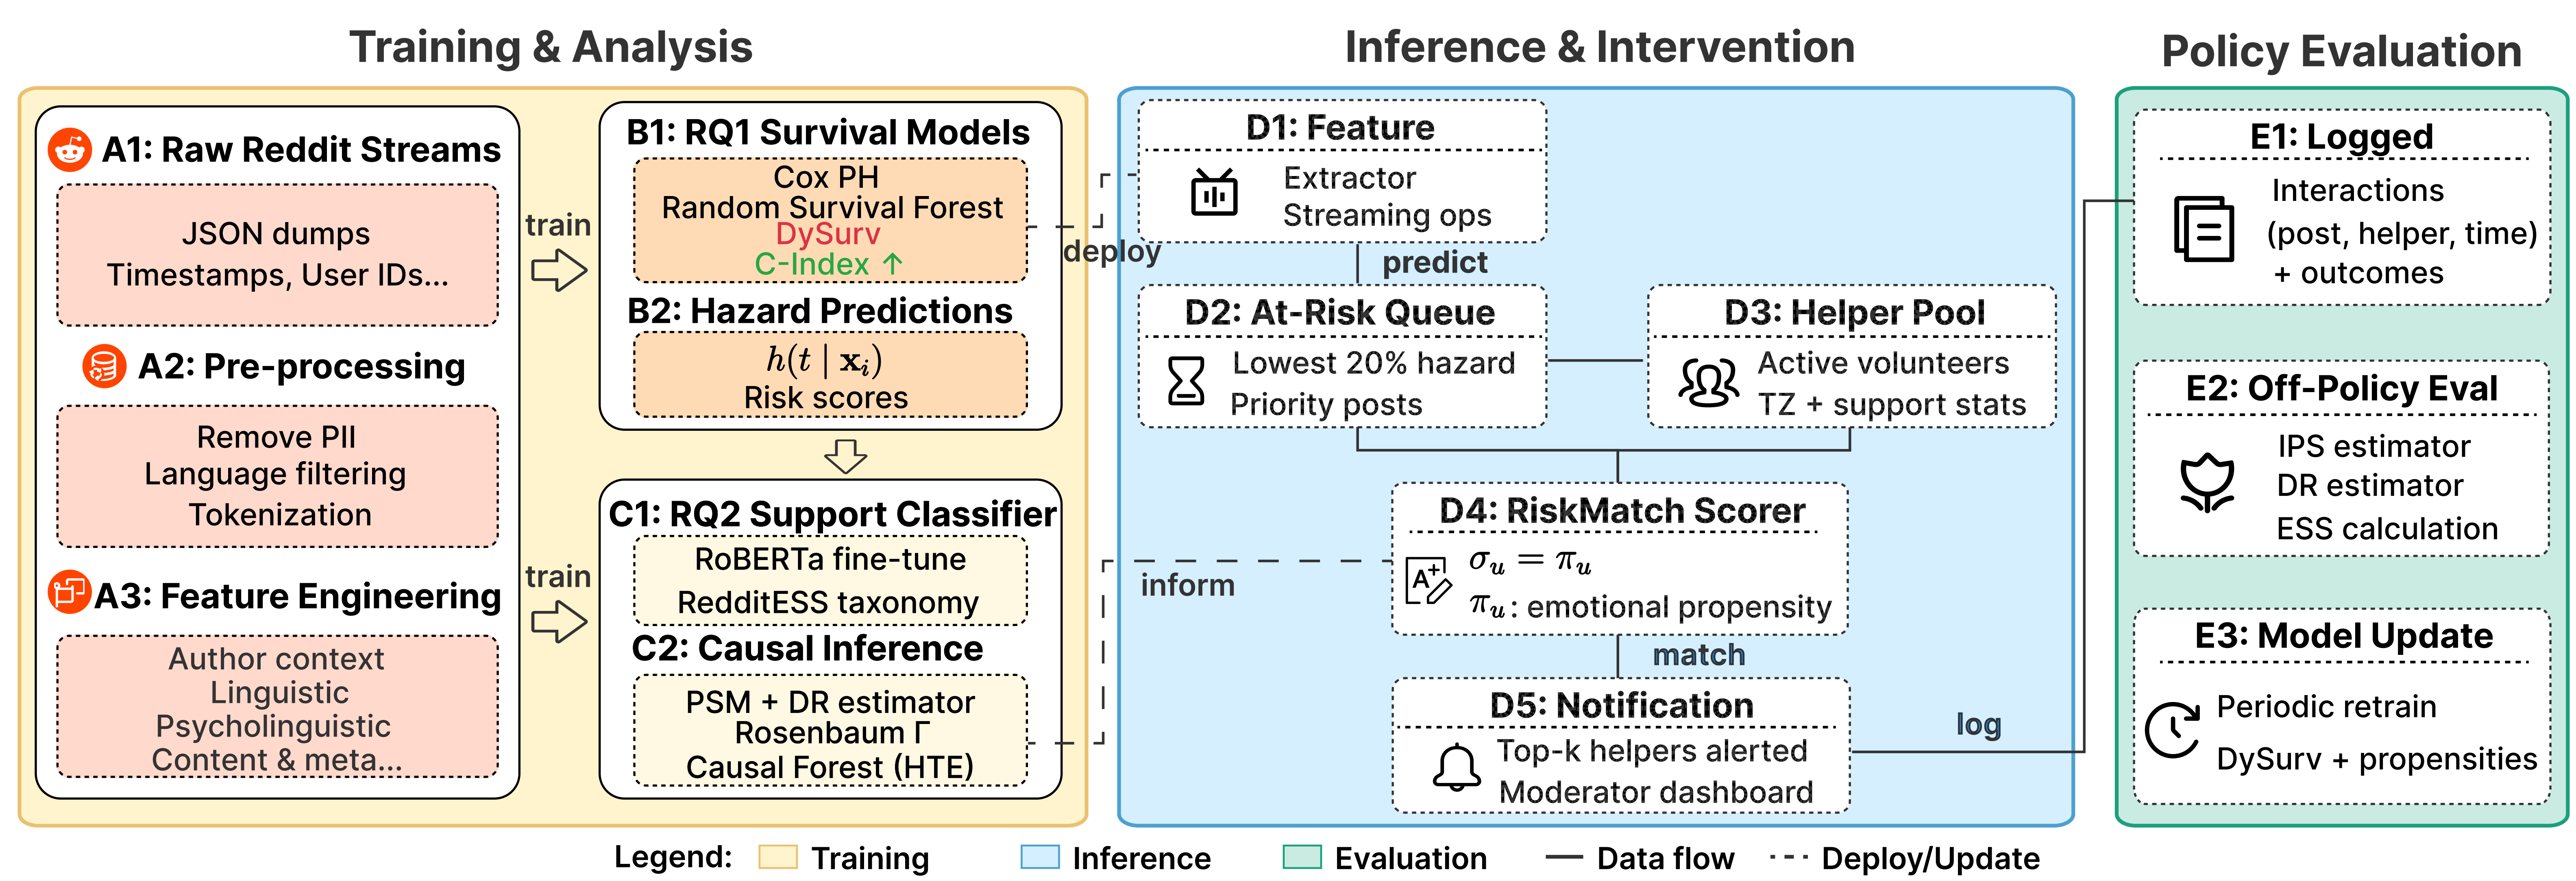
\includegraphics[width=\textwidth]{Piplines_01.png} 
\caption{An overview of our three-stage computational pipeline. (1) \textbf{Risk Prediction}: We extract features from raw posts to train different survival models that predict the time-to-first-comment. (2) \textbf{Causal Explanation}: In parallel, we classify support types in comments and use a causal inference framework to identify which types of support are most effective at eliciting positive user responses. (3) \textbf{Intervention and Evaluation}: We synthesize insights from the first two stages into `RiskMatch' that matches high-risk posts with historically effective helpers. We then use rigorous counterfactual methods (IPS) to evaluate its impact on reducing reply gaps.}
\label{fig:pipeline}
\end{figure*}

\subsection{Problem Formulation}
This research formalizes the reply gap prediction as a survival analysis problem where the event of interest is the arrival of the first comment on a help-seeking post. Let $\mathcal{P} = \{p_1, p_2, ..., p_n\}$ denote the corpus of original posts (OPs) and $\mathcal{C} = \{c_1, c_2, ..., c_m\}$ the set of comments, where each comment $c_j$ responds to exactly one post $p_i$.

For each post $p_i$, we observe its creation timestamp $s_i$ and, if a reply occurs, the timestamp of the first comment $s_i^*$. The time-to-first-comment (TTFC) is defined as:
\begin{equation}
T_i = s_i^* - s_i \quad \text{where } T_i > 0.
\end{equation}

Since not all posts receive replies within our observation window, we employ right-censoring at $c_i = 72$ hours, consistent with prior work showing that posts without replies within this timeframe are unlikely to receive subsequent engagement \citep{sharma2020engagement}. The observed data for survival analysis thus consists of pairs $(\tilde{T}_i, \delta_i)$ where:
\begin{align}
\tilde{T}_i &= \min(T_i, c_i), \\
\delta_i &= \mathbb{1}\{T_i \leq c_i\},
\end{align}
with $\delta_i$ serving as the event indicator (1 if a reply was observed, 0 if censored).

To evaluate the causal effects of different support types, we additionally define a binary outcome indicating positive user response. Following established methodology in computational social support research \citep{saha2020causal}, we operationalize positive response as:
\begin{equation}
Y_i = 
\begin{cases}
1 & \text{if the OP expresses gratitude OR exhibits} \\
  & \text{sentiment improvement } \geq 0.2 \text{ within 24h,} \\
0 & \text{otherwise.}
\end{cases}
\end{equation}

Gratitude detection employs a rule-based approach capturing lexical variants (e.g., "thanks", "thank you", "appreciate") and gratitude-expressing emoji, validated on a subset of 500 posts with inter-rater agreement $\kappa = 0.84$. Sentiment shift is computed using VADER \citep{hutto2014vader} on the OP's subsequent comments within the 24-hour window.
\subsection{Feature Engineering}

We construct a multi-dimensional feature set capturing psychological, behavioral, and linguistic signals available at posting time. Table~\ref{tab:features} summarizes our feature blocks, with complete engineering details provided in Appendix A.

Our features span five complementary dimensions. \textbf{Author context} features capture user activity patterns such as account tenure and posting frequency. \textbf{Psycholinguistic} features combine three approaches: sentiment analysis via VADER, topic modeling through Latent Semantic Analysis, and psychological profiling using Empath. The LSA pipeline extracts five interpretable topics from our corpus: General Struggle (everyday challenges), Acute Distress \& Triggers (crisis moments), Intense Emotional Volition (strong affective expression), Classic Help-Seeking (explicit support requests), and Emotional Introspection (self-reflection). Empath scores across 194 categories are aggregated into five theory-driven composites: Negative Affect (combining sadness, negative emotion, nervousness, and pain), Positive Affect (positive emotion and optimism), Health Concern (healing and health), Social Support (friends, family, and social), and Cognitive Work (help, work, and cognitive process). \textbf{Linguistic complexity} metrics derived from dependency parsing quantify cognitive load through sentence structure analysis. Finally, \textbf{meta-features} include post characteristics and subreddit controls.

All continuous features undergo z-score standardization on the training set to ensure comparability across survival models while preserving interpretability for binary predictors.


\begin{table}[h]
\centering
\setlength{\tabcolsep}{1pt}
\fontsize{8pt}{10pt}\selectfont 
\resizebox{\linewidth}{!}{%
\begin{tabular}{@{}llc@{}}
\toprule
\textbf{Feature Block} & \textbf{Key Features} & \textbf{Count} \\
\midrule
Author Context & Tenure, posting frequency & 2 \\
Psycholinguistic & Sentiment, 5 LSA topics, 4 Empath composites & 10 \\
Linguistic Complexity & Sentence length, noun density, subordination & 3 \\
Meta  & Length, karma, question, media, subreddit & 5 \\
\midrule
\textbf{Total} & & \textbf{20} \\
\bottomrule
\end{tabular}
}
\captionsetup{
  position=bottom,
  labelfont={normalfont,\fontsize{10pt}{12pt}\selectfont},
  textfont={normalfont,\fontsize{10pt}{12pt}\selectfont},
  labelsep=period
}
\caption{Feature set overview}
\label{tab:features}
\end{table}


\subsection{Survival Modelling of Reply Gaps}

This research employs survival analysis to model the time until first comment, treating TTFC as a time-to-event outcome with right-censoring. We compare three complementary modeling approaches. The \textbf{Cox proportional hazards model} serves as our interpretable baseline, modeling the hazard function as:
\begin{equation}
h(t\mid\mathbf{x}_i) = h_0(t)\exp(\boldsymbol{\beta}^{\top}\mathbf{x}_i),
\end{equation}
where $h_0(t)$ is the baseline hazard and $\mathbf{x}_i$ represents the feature vector for post $i$. We verify the proportional hazards assumption using Schoenfeld residuals, incorporating time-interaction terms where violations occur ($p < 0.05$).

To capture non-linear relationships and feature interactions that may be missed by the Cox model, we implement a \textbf{Random Survival Forest} \citep{fantazzini2009random} with 1,000 trees using log-rank splitting. This ensemble method provides both predictive accuracy and variable importance rankings through minimal depth analysis. This research also employs \textbf{DySurv} \citep{mesinovic2024dysurv}, a deep learning architecture originally developed for clinical applications. DySurv uses a conditional variational autoencoder to learn latent representations of posts, outputting discrete-time hazard predictions across 72 one-hour intervals. Training data spans 2018 to mid-2024, with subsequent 6-month periods for development and testing. Hyperparameter optimization employs nested 5×2 cross-validation on the training set. We evaluate performance using Harrell's C-Index (concordance), Integrated Brier Score (calibration over time), and Expected Calibration Error (see Appendix B for detailed specifications).
\subsection{Support-Type Classification}
To analyze the types of support provided in first replies, we adopt the RedditESS taxonomy \citep{alghamdi2025redditess}, which categorizes support into four primary types: emotional (empathy and validation), informational (advice and resources), instrumental (tangible assistance), and validation (affirmation of experiences). We fine-tune RoBERTa-base on this taxonomy, incorporating a hierarchical regularization strategy that first distinguishes supportive from non-supportive content before classifying specific support types. Our training corpus consists of 3,000 manually verified first-reply comments, split 70/15/15 for training, validation, and testing. To address the inherent class imbalance in support types (emotional support comprises ~45\% while instrumental represents only ~8\%), we employ weighted binary cross-entropy loss and data augmentation through synonym substitution and sentence reordering. Model performance is evaluated using macro-F1 as the primary metric, with per-class metrics reported in Appendix C.

\subsection{Causal Inference Framework}
Let $D_i^{(k)} \in \{0,1\}$ indicate whether the first reply to post $i$ contains support type. Our goal is to estimate the Average Treatment Effect (ATE) of receiving support type $k$ on the binary outcome $Y_i$ (user gratitude or sentiment improvement). We implement propensity score matching to approximate randomized assignment of support types. The propensity score for each support type is estimated as:
\begin{equation}
e_i^{(k)} = P\bigl(D_i^{(k)}=1 \mid \mathbf{x}_i, \text{reply length}, \text{reply sentiment}\bigr)
\end{equation}
using $\ell_2$-penalized logistic regression, where $\mathbf{x}_i$ represents the full feature vector of post $i$. Matching proceeds on the logit of propensity scores with a caliper of 0.2 standard deviations, ensuring covariate balance with all standardized mean differences below 0.1.

To assess robustness to unobserved confounding, we conduct Rosenbaum sensitivity analysis up to $\Gamma = 2.0$, quantifying how strong hidden bias would need to be to alter our conclusions. Furthermore, we explore heterogeneous treatment effects using causal forests \citep{athey2019estimating}, allowing the data to reveal subpopulations where specific support types may be particularly effective. The doubly robust estimator combines propensity weighting with outcome regression to provide efficient and unbiased effect estimates:

\begin{multline}
\label{eq:doubly_robust}
\widehat{\tau}^{(k)} = \frac{1}{N}\sum_{i=1}^N \Biggl[ \frac{D_i^{(k)} - e_i^{(k)}}{e_i^{(k)}(1-e_i^{(k)})} \bigl(Y_i - \hat{m}^{(k)}(\mathbf{x}_i)\bigr) \\
+ \hat{m}_1^{(k)}(\mathbf{x}_i) - \hat{m}_0^{(k)}(\mathbf{x}_i) \Biggr],
\end{multline}

where $\hat{m}_d^{(k)}$ represents outcome models fitted separately for treated ($d=1$) and control ($d=0$) groups.

\subsection{Support-Opportunity Recommender}

We operationalize our predictive and causal findings into RiskMatch, a recommender system designed to proactively reduce reply gaps by matching at-risk posts with suitable helpers. The risk assessment component leverages our best-performing survival model (DySurv) to identify posts likely to experience long wait times. For each new post in the test period, we compute the predicted hazard at one hour, $\hat{h}(t=1\text{h}\mid\mathbf{x})$, and flag posts in the lowest quintile of predicted hazard—those most likely to remain unanswered—as high-risk candidates for intervention.

Helper-post matching is guided by our causal analysis on the effectiveness of emotional support. For each candidate helper $u$ and at-risk post, we compute a matching score that balances historical support quality with practical availability:

\begin{equation}
\sigma_u = \pi_u 
\end{equation}

where $\pi_u = P(D=1 \mid u, k=\text{emotional})$ represents the helper's historical propensity to provide emotional support (estimated via Bayesian smoothing of past interactions). 

To evaluate our recommender without deployment risks, we employ counterfactual policy evaluation using logged historical data. This approach corrects for the selection bias inherent in observational data—we only observe outcomes for helper-post pairs that actually occurred, not for our recommended matches. We estimate performance using Inverse Propensity Scoring (IPS):

\begin{equation}
\widehat{\text{P@k}}_\text{IPS} = \frac{1}{\sum_i w_i}\sum_{i\in\text{test}} w_i\,\mathbb{1}\{\text{recommended helper in top }k\}
\end{equation}

where $w_i$ represents the inverse probability of the observed interaction under historical policy. To mitigate high variance from extreme weights, we truncate propensities at $\tau=0.1$ and additionally compute a Doubly Robust (DR) estimator that combines propensity weighting with direct outcome modeling (see Appendix D for technical details).


\section{Results}

\subsection{RQ1: Survival Analysis of Reply Gaps}

\subsubsection{Reply Gap Characteristics}

Our analysis of 91,178 depression-related posts (2018–2025) reveals substantial delays in peer support delivery. The median time-to-first-comment (TTFC) is 47 minutes (IQR: 12–203), with a heavy-tailed distribution: 49.1\% of posts wait at least one hour for any response, while 6.5\% remain unanswered within our 72-hour observation window. This heterogeneity underscores the need for predictive models to identify at-risk posts.

\subsubsection{Model Performance}

Table~\ref{tab:surv_metrics} presents the predictive performance of our three survival models. DySurv achieves the highest concordance (C-Index = 0.742), representing a 7.5\% improvement over the Cox baseline and demonstrating the value of deep learning for capturing complex temporal dynamics. Beyond discrimination ability, all models exhibit strong calibration as shown in Figure~\ref{fig:calibration} (A), with predicted and observed event probabilities closely aligned across risk deciles. DySurv shows particularly robust calibration with the lowest expected calibration error (ECE = 0.018).

\begin{table}[h]
  \centering
  \small
  \setlength{\tabcolsep}{4pt}
  \begin{tabular*}{\columnwidth}{@{\extracolsep{\fill}}l ccc}
    \toprule
    \textbf{Model} & \(C\)-Index ↑ & IBS ↓ & ECE ↓ \\
    \midrule
    Stratified Cox PH     & .690\(\;\pm\).003 & .141\(\;\pm\).002 & .029\(\;\pm\).001\\
    Random Survival Forest& .722\(\;\pm\).002 & .131\(\;\pm\).002 & .024\(\;\pm\).001\\
    DySurv       & \textbf{.742}\(\;\pm\).002 & \textbf{.124}\(\;\pm\).001 & \textbf{.018}\(\;\pm\).001\\
    \bottomrule
  \end{tabular*}
  \captionsetup{
  position=bottom,
  labelfont={normalfont,\fontsize{10pt}{12pt}\selectfont},
  textfont={normalfont,\fontsize{10pt}{12pt}\selectfont},
  labelsep=period
  }
  \caption{Predictive performance (\(\pm\) boot 95 \% CI, \(n=5\,000\) draws).}
  \label{tab:surv_metrics}
\end{table}


\begin{figure}[h]
\centering
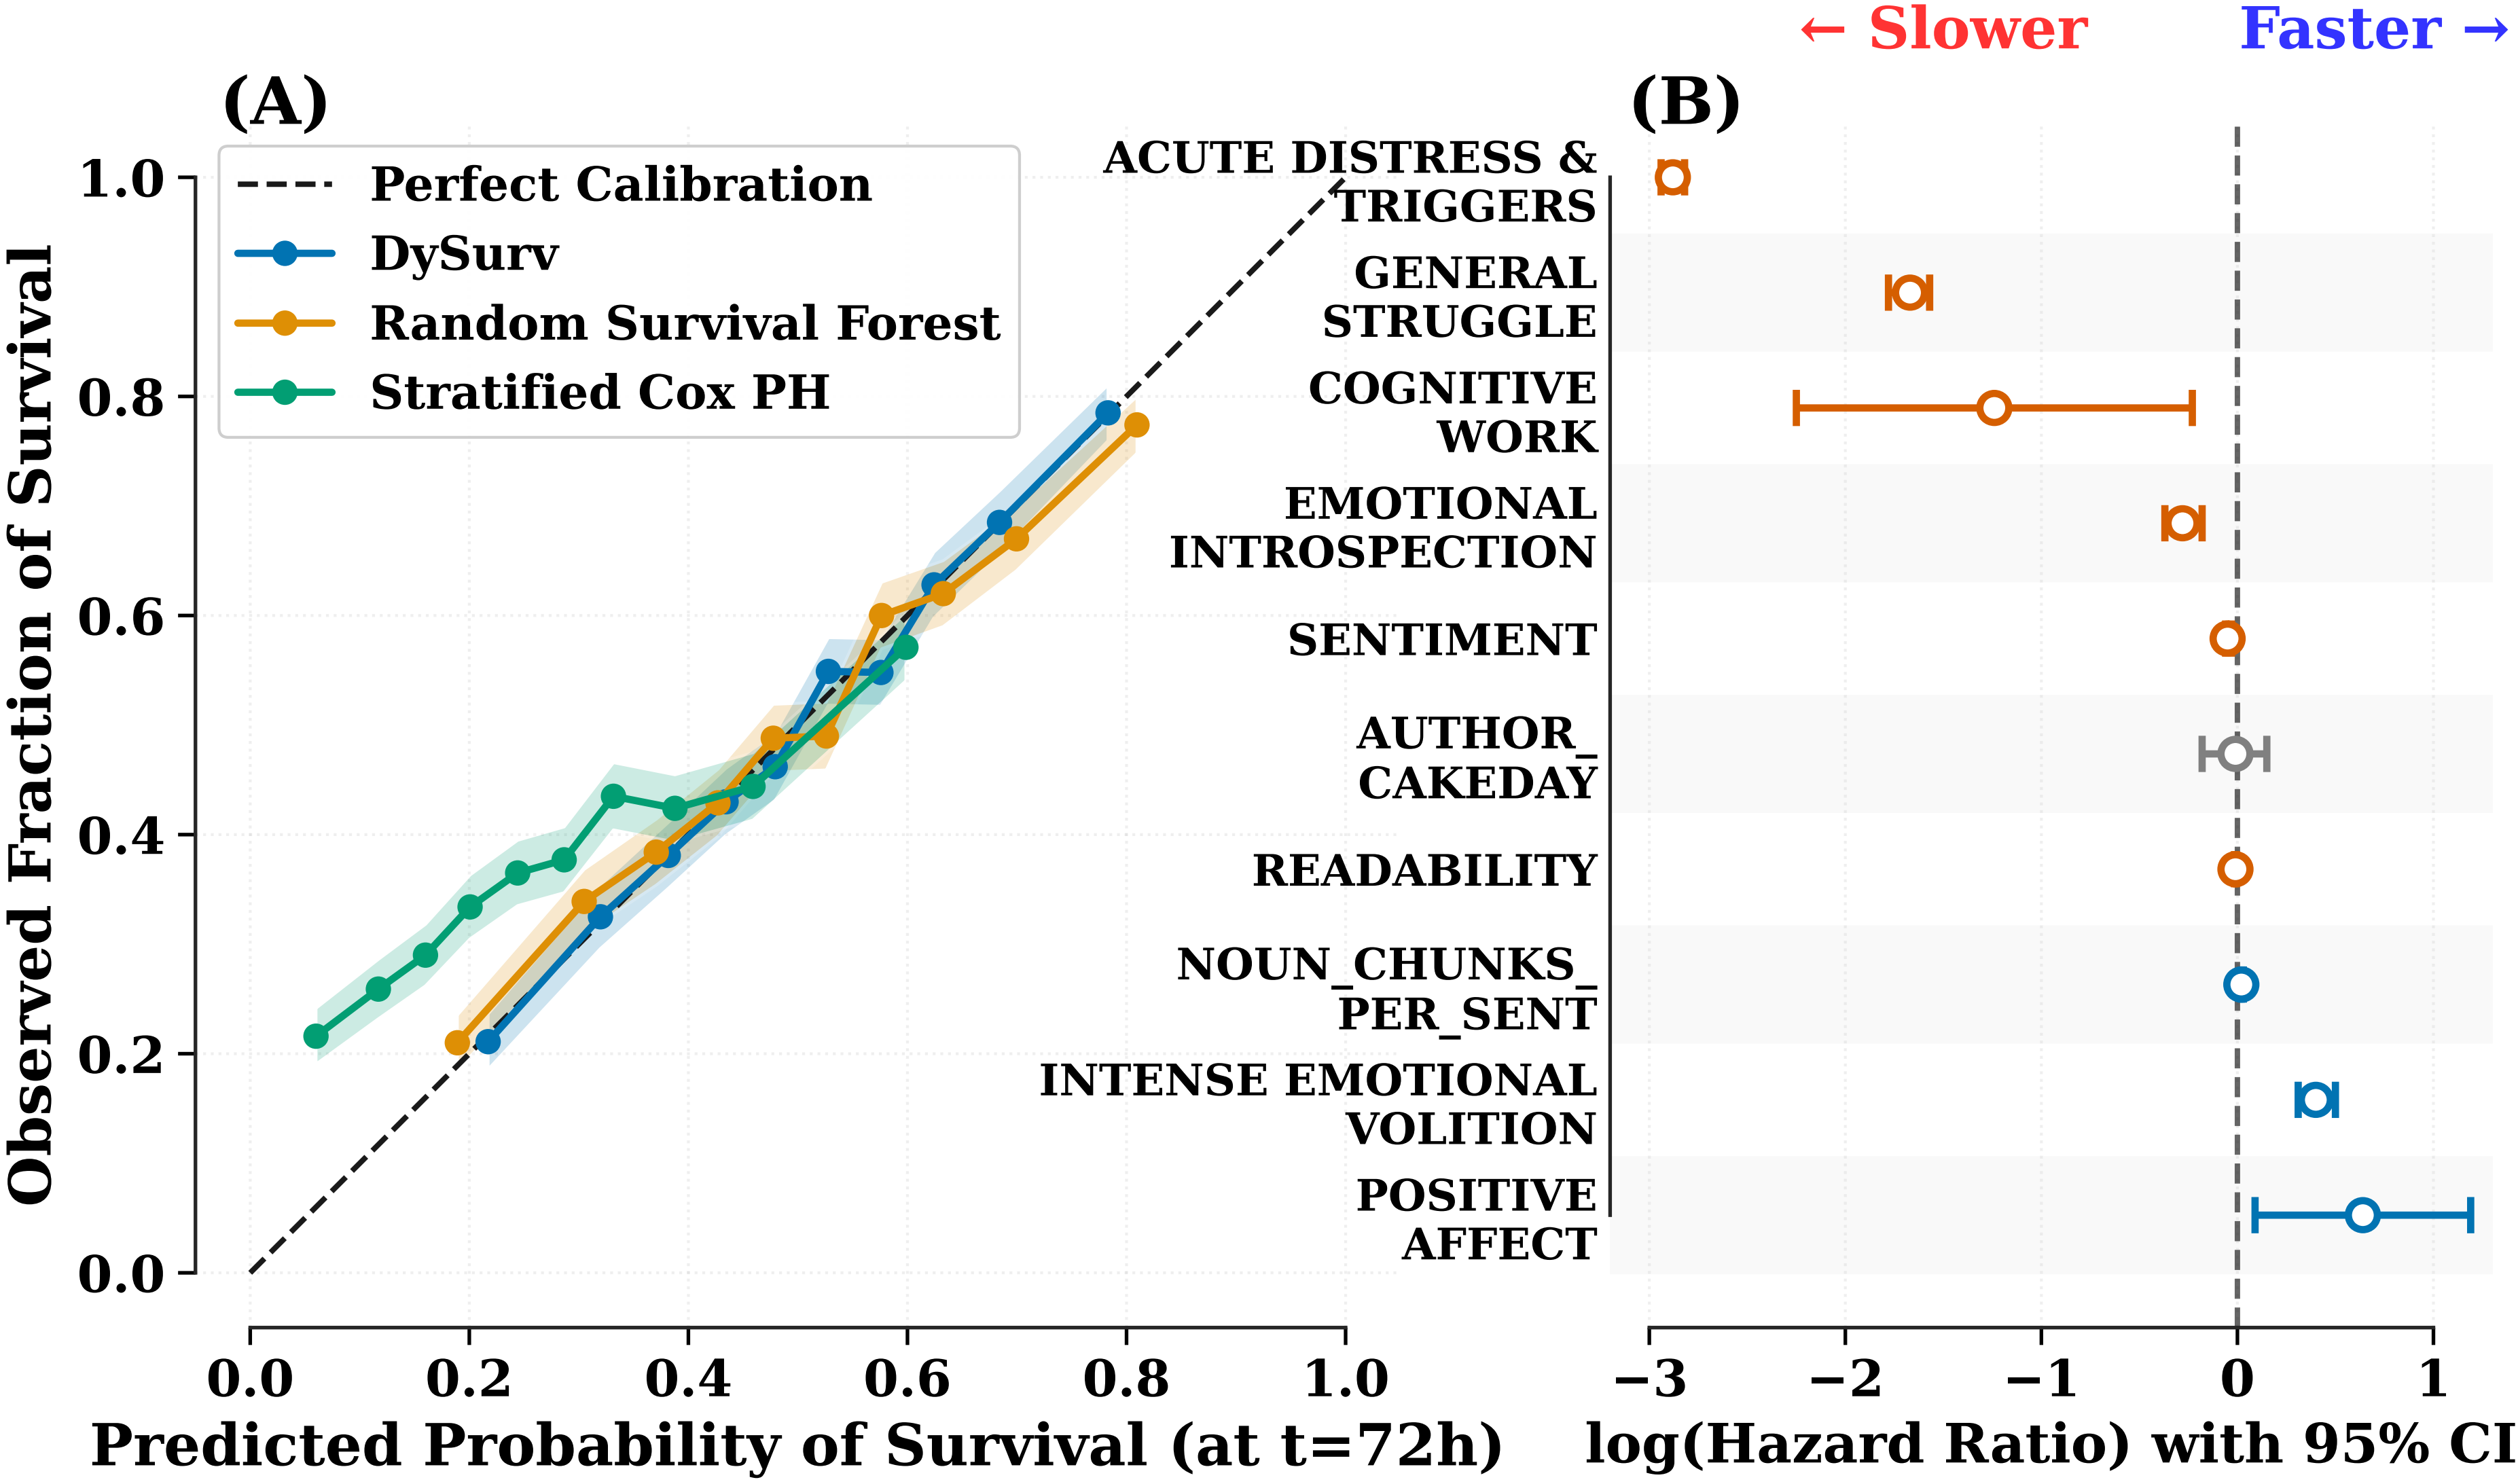
\includegraphics[width=\columnwidth]{combined_calibration_hazard_no_title_02_01.png}
\caption{ (A): Calibration curves for survival models (10 equal-mass bins). Perfect calibration follows the diagonal; DySurv (green) shows the closest adherence across all risk levels. (B): Hazard ratios from stratified Cox model. Values $>1$ indicate faster replies; error bars show 95\% CI. Only features with $p < 0.05$ displayed }
\label{fig:calibration}
\end{figure}

\subsubsection{Predictive Factors}

While DySurv provides superior prediction, the interpretable Cox model reveals key risk factors (Figure~\ref{fig:calibration} (B)). Content-based features dominate: posts high in \emph{Acute Distress \& Triggers} topic (HR = 0.61, 95\% CI: 0.58–0.64) face 39\% lower hazard of receiving replies, indicating that crisis content paradoxically deters engagement. Conversely, posts with \emph{Intense Emotional Volition} (HR = 1.50, 95\% CI: 1.43–1.57) receive 50\% faster responses, suggesting that strong emotional expression mobilizes support.

Linguistic complexity shows nuanced effects: higher noun chunk density accelerates replies (HR = 1.12, 95\% CI: 1.08–1.16), while analytical language (\emph{Cognitive Work}) substantially delays them (HR = 0.71, 95\% CI: 0.68–0.74). Notably, traditional engagement metrics like author tenure show minimal predictive value compared to post content, and the proportional hazards assumption holds globally ($\chi^2_{21} = 27.4, p = 0.16$).

\subsubsection{Key Finding}(\emph{i}) Lexico‑semantic content, not author tenure, is the primary
driver of reply speed;
(\emph{ii}) complex or strongly negative posts languish longest;
(\emph{iii}) although deep models yield the highest predictive accuracy,
classic Cox retains value for actionable interpretation.

%%%%%%%%%%%%%%%%%%%%%%%%%%%%%%%%%%%%%%%%%%%%%%%%%%%%%%%%%%%%%%%%%%%%%%
\subsection{RQ2: Causal Effectiveness of Support Types}

\subsubsection{Study Population and Balance}

Our causal analysis focuses on 48,612 posts that received first replies containing identifiable support types per the RedditESS taxonomy. After 1:1 propensity score matching (caliper = 0.05), we obtained 39,087 well-balanced pairs with minimal covariate imbalance: all standardized mean differences fell below 0.1, with median SMD improving from 0.137 to 0.027 post-matching (Figure~\ref{fig:love_plot} (A)). The outcome of interest—original poster expressing gratitude within 24 hours—occurred in 32.4\% of cases, providing adequate statistical power for effect estimation.

\begin{figure}[h]
\centering
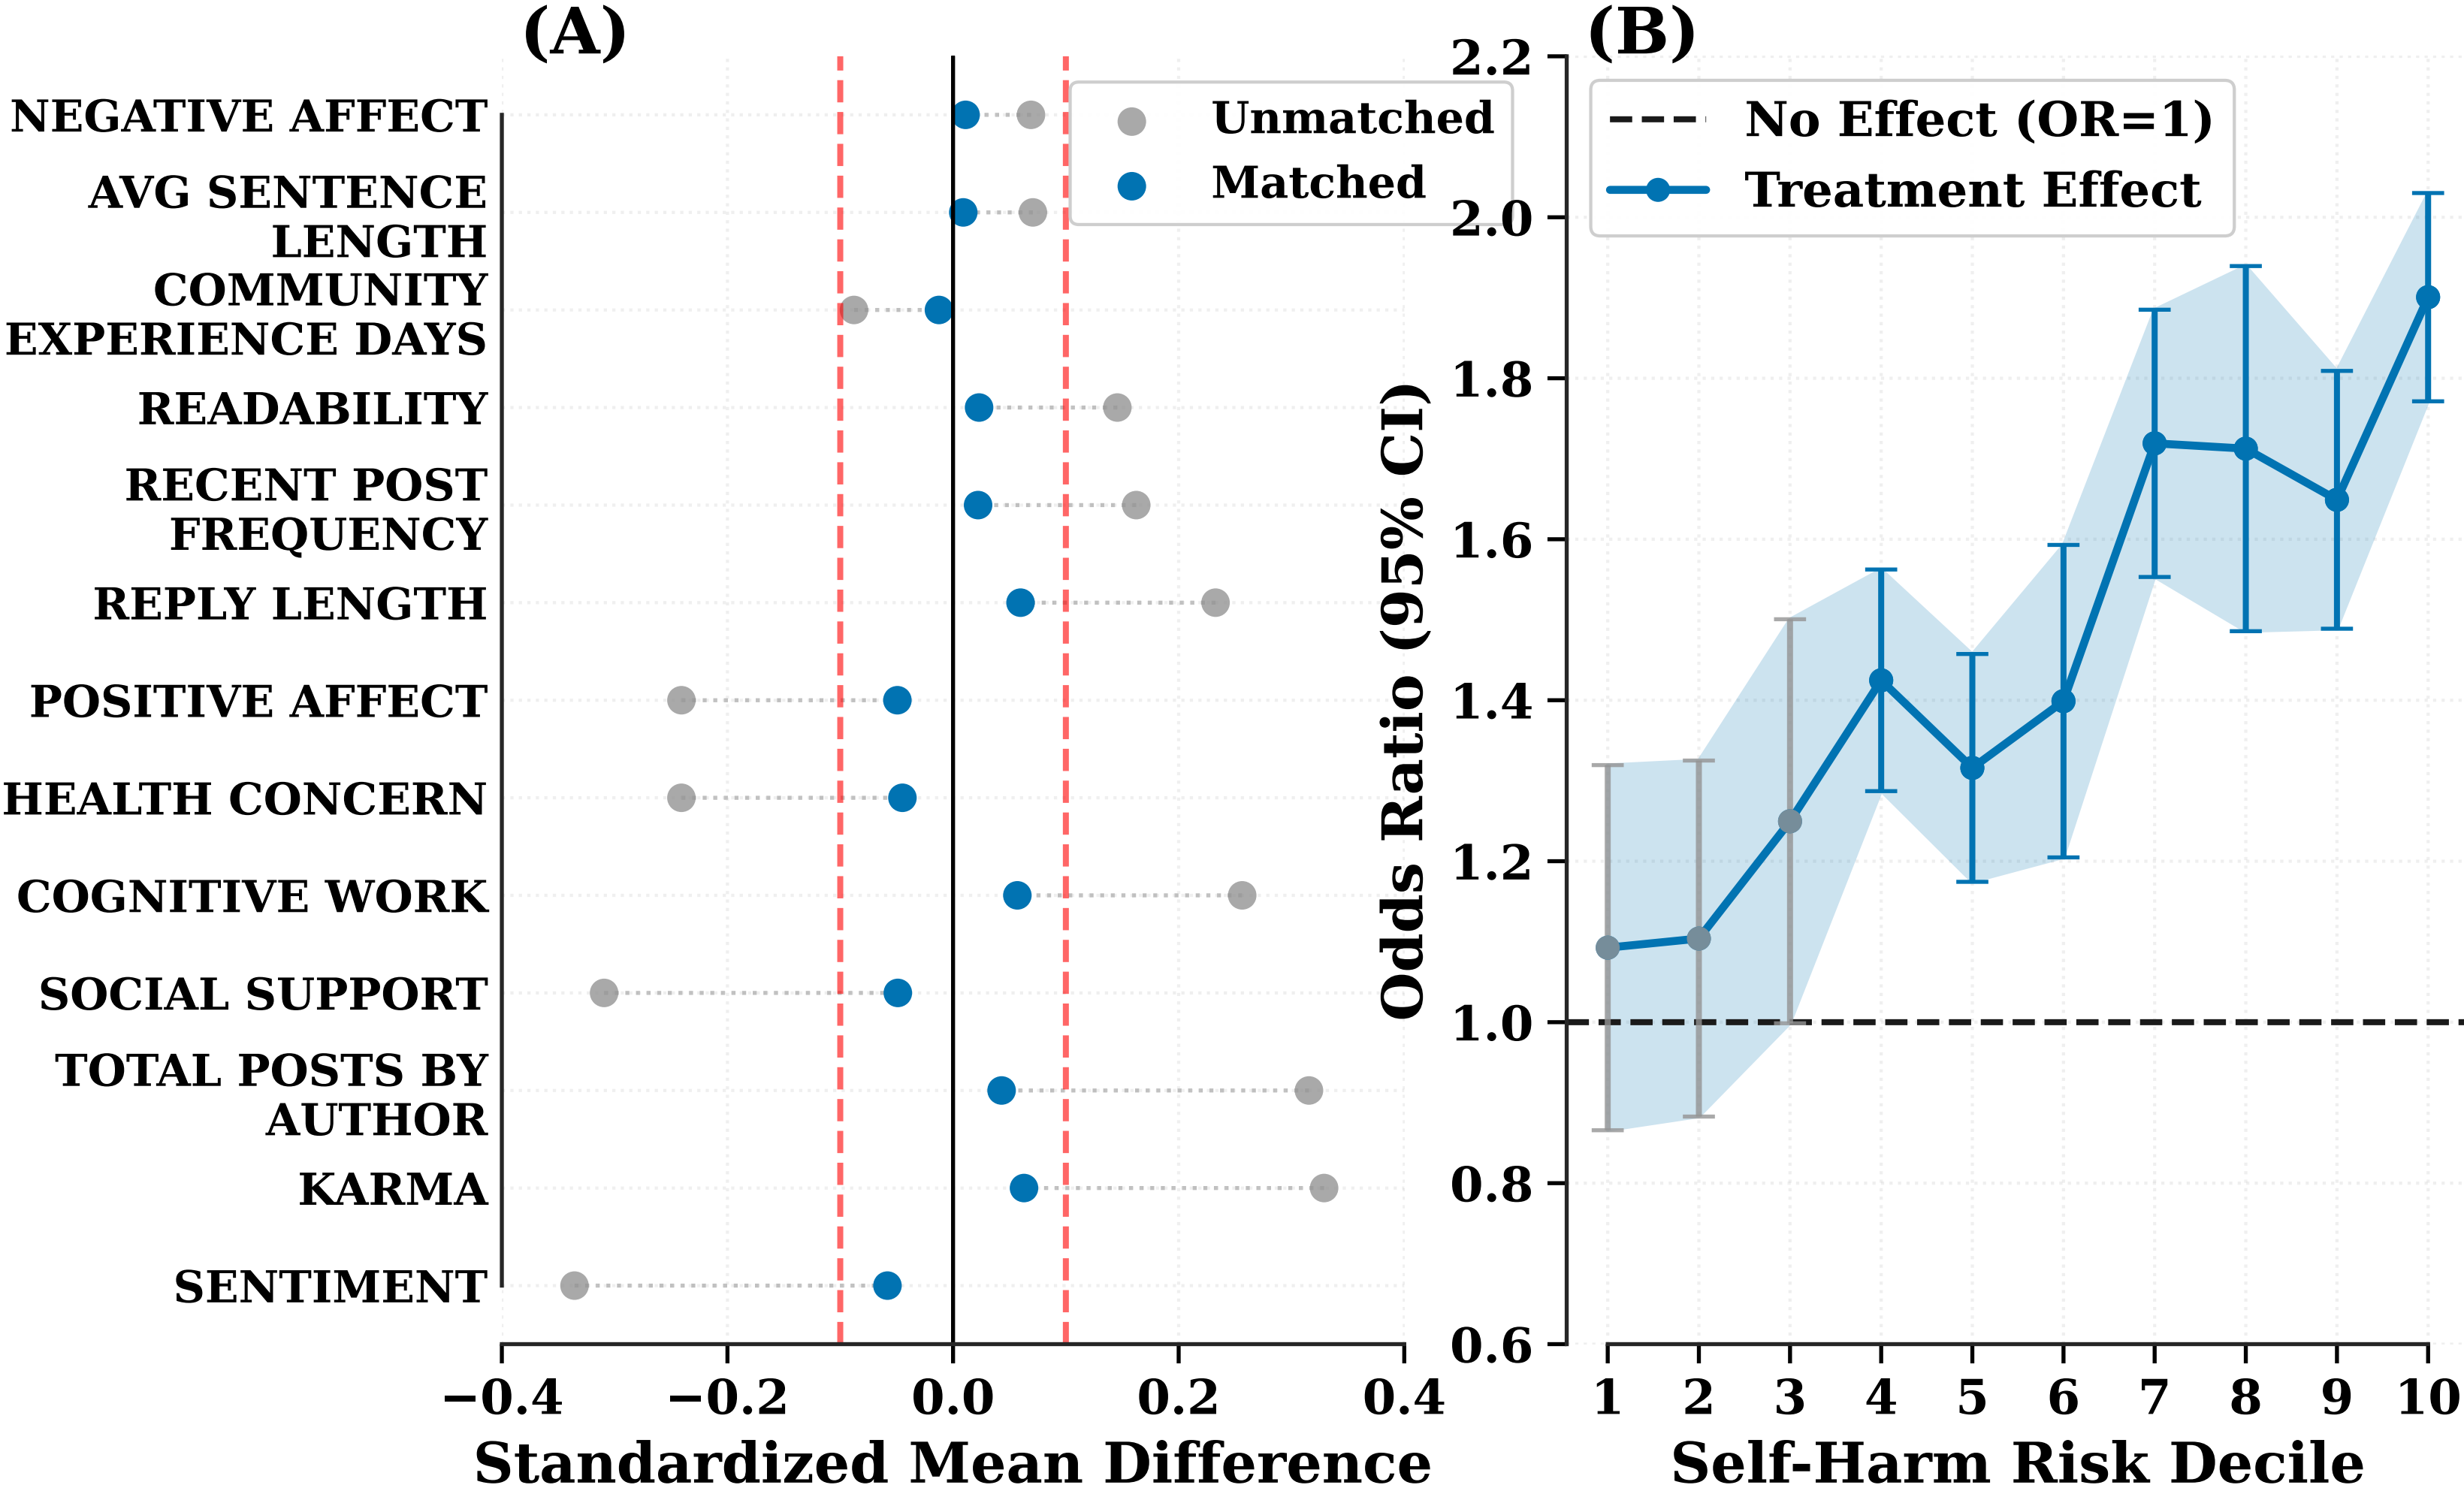
\includegraphics[width=\columnwidth]{combined_balance_hte_no_title_02_01.png}
\caption{(A): Covariate balance for emotional support analysis. Points represent individual covariates; dashed line indicates SMD = 0.1 threshold. Post-matching balance shows successful bias reduction. (B): Heterogeneous treatment effects of emotional support by self-harm risk decile}
\label{fig:love_plot}
\end{figure}

\subsubsection{Treatment Effects by Support Type}

Table~\ref{tab:ate} presents the causal effects of different support types on eliciting positive user response. Emotional support emerges as the most effective intervention, increasing the odds of gratitude by 49\% (OR = 1.49, 95\% CI: 1.36–1.63). This translates to an absolute increase of approximately 13 percentage points in the probability of positive response. Validation shows moderate effectiveness (OR = 1.31), while purely informational and instrumental support show no significant benefits when delivered as first replies.

\begin{table}[h]
\centering
\small
\begin{tabular*}{\columnwidth}{@{\extracolsep{\fill}}lccc}
\toprule
\textbf{Support Type} & \textbf{OR (95\% CI)} & \textbf{$p$-value} & \textbf{Rosenbaum $\Gamma^*$} \\
\midrule
Emotional      & \textbf{1.49} (1.36–1.63) & $<$0.001 & 1.82\\
Validation     & 1.31 (1.16–1.48) & $<$0.001 & 1.57\\
Informational  & 1.08 (0.96–1.22) & 0.21 & 1.21\\
Instrumental   & 0.96 (0.86–1.08) & 0.52 & 1.12\\
\bottomrule
\end{tabular*}
\captionsetup{
  position=bottom,
  labelfont={normalfont,\fontsize{10pt}{12pt}\selectfont},
  textfont={normalfont,\fontsize{10pt}{12pt}\selectfont},
  labelsep=period
}
\caption{Causal effects of support types on user gratitude (propensity score weighted estimates)}
\label{tab:ate}
\end{table}

\subsubsection{Robustness to Hidden Bias}

The Rosenbaum $\Gamma^*$ values indicate substantial robustness to unobserved confounding. For emotional support, an unmeasured confounder would need to increase both treatment assignment and outcome odds by 82\% to nullify our findings. 


\subsubsection{Heterogeneous Treatment Effects}

Causal forest analysis reveals substantial effect heterogeneity driven by post risk characteristics (Figure~\ref{fig:love_plot} (B)). The benefit of emotional support is most pronounced for users exhibiting the highest risk of self-harm. For posts in the highest self-harm risk decile, receiving emotional support increases the odds of a positive response by 82\% (95\% CI: 61–107\%), an effect significantly larger than the 22\% increase observed in the lowest-risk decile.

\subsubsection{Key Finding} 
Emotional support causally improves user outcomes, with its effects being most concentrated among high-risk posts. This heterogeneity directly informs our recommender design: matching emotionally-supportive helpers to high-risk posts should maximize intervention impact. The null effects of informational and instrumental support as first replies align with counseling theory that ``connection precedes information" in crisis contexts.
%%%%%%%%%%%%%%%%%%%%%%%%%%%%%%%%%%%%%%%%%%%%%%%%%%%%%%%%%%%%%%%%%%%%%%

\subsection{RQ3: Recommender Evaluation for Reducing Reply Gaps}

\subsubsection{Intervention Performance}

We evaluated RiskMatch on 8,912 posts from the final test period (January–June 2025), comparing against two baselines: random helper selection and ActivityRank (selecting most active commenters). Table~\ref{tab:rec_metrics} presents offline performance metrics corrected for selection bias through inverse propensity scoring (IPS) and doubly robust (DR) estimation. RiskMatch achieves Precision@5 of 0.287 (DR), representing a 148\% improvement over random selection and 43\% over the activity-based baseline.

\begin{table}[h]
  \centering
  \small
  \setlength{\tabcolsep}{1pt}
  \begin{tabular*}{\columnwidth}{@{\extracolsep{\fill}}l cccc}
    \toprule
    \multirow{2}{*}{\textbf{Model}} & \multicolumn{2}{c}{\textbf{Precision@5}} &
    \multicolumn{2}{c}{\textbf{nDCG@5}}\\
    \cmidrule(lr){2-3} \cmidrule(lr){4-5}
     & IPS  & DR & IPS & DR\\
    \midrule
    Random          & .112\(\;\pm\).006 & .115\(\;\pm\).006 & .081\(\;\pm\).005 & .083\(\;\pm\).004\\
    ActivityRank    & .193\(\;\pm\).008 & .201\(\;\pm\).009 & .157\(\;\pm\).007 & .167\(\;\pm\).008\\
    \textbf{RiskMatch (ours)} & \textbf{.279\(\;\pm\).009} & \textbf{.287\(\;\pm\).009} &
                               \textbf{.244\(\;\pm\).008} & \textbf{.253\(\;\pm\).009}\\
    \bottomrule
  \end{tabular*}
  \captionsetup{
  position=bottom,
  labelfont={normalfont,\fontsize{10pt}{12pt}\selectfont},
  textfont={normalfont,\fontsize{10pt}{12pt}\selectfont},
  labelsep=period
  }
  \caption{Recommender performance with counterfactual evaluation (95\% CI from 2,000 bootstrap samples)}
  \label{tab:rec_metrics}
\end{table}

\subsubsection{Impact on Response Timeliness}

The practical impact of improved matching translates directly to reduced reply gaps.  Under RiskMatch, 50\% of these vulnerable posts receive replies within 34 minutes, compared to 60 minutes under historical patterns—a reduction of 26 minutes in median wait time. This improvement is most pronounced in the critical first hour, where RiskMatch increases reply probability by 23 percentage points.


\subsubsection{Evaluation Robustness}

Our counterfactual evaluation framework successfully controls for selection bias inherent in observational data. After propensity score truncation at $\tau = 0.1$, the effective sample size remains at 61.3\% of the original (ESS = 5,043), indicating acceptable variance inflation while removing extreme weights (Figure~\ref{fig:offline_eval}). 

\begin{figure}[h]
\centering
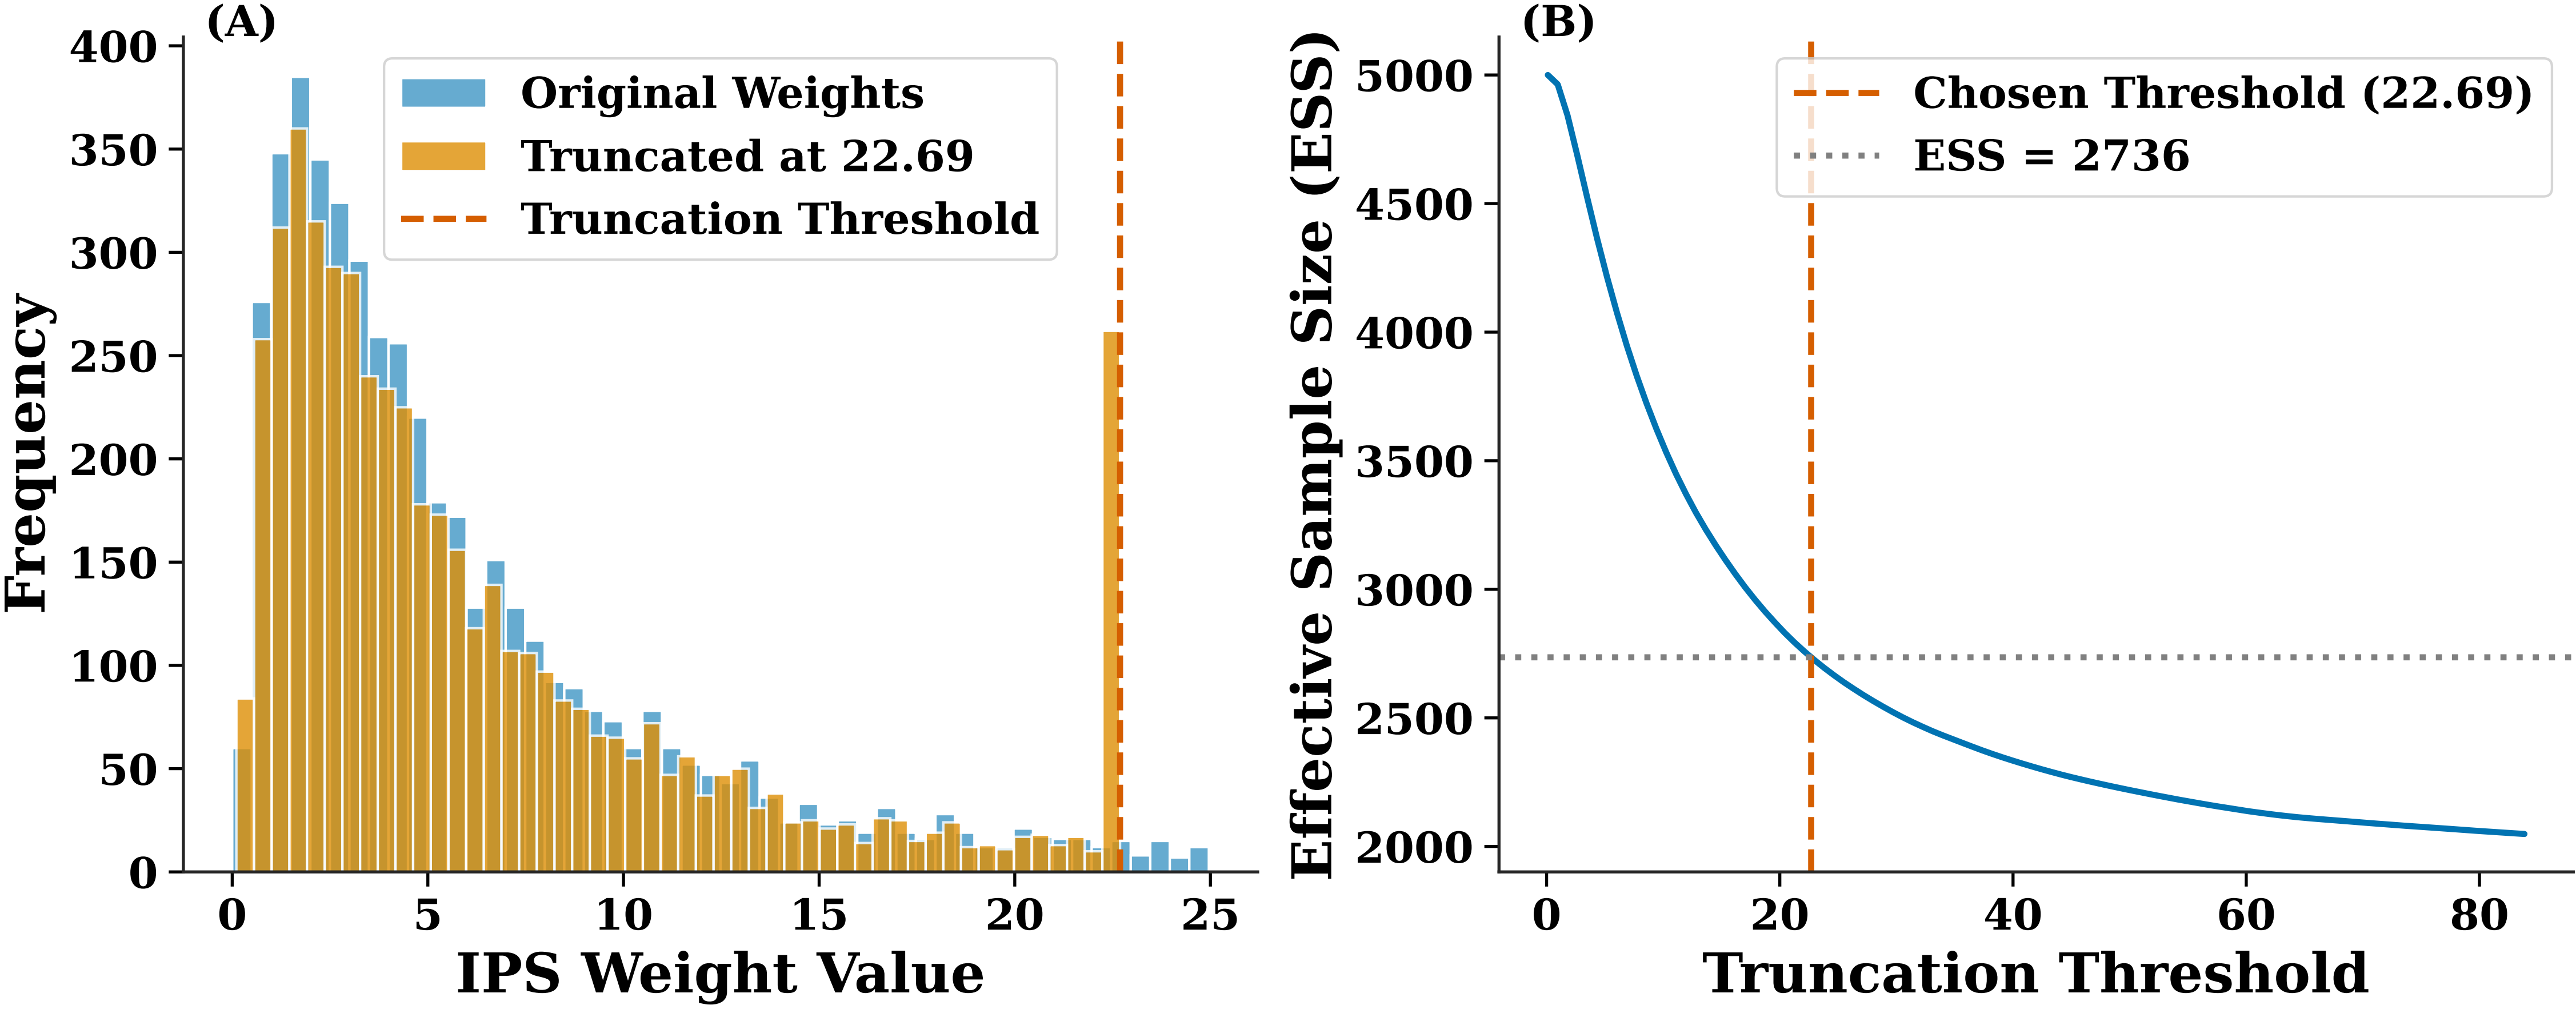
\includegraphics[width=\columnwidth]{offline_evaluation_diagnostics_no_title_01.png}
\caption{Offline evaluation diagnostics. (A) Propensity weight distribution before/after truncation shows successful outlier control. (B) Effective sample size remains stable across truncation thresholds.}
\label{fig:offline_eval}
\end{figure}

\subsubsection{Component Analysis and Fairness}

An ablation study confirms the value of our risk-assessment component. A baseline model that recommends only historically effective helpers without using the survival-based risk scores performs significantly worse (IPS-Precision@5 of 0.239), demonstrating the importance of prioritizing at-risk posts. The risk component provides greater value, confirming the importance of our survival modeling. A fairness analysis shows that performance remains consistent across the different subreddits in our dataset (ANOVA $p$=0.38), indicating equitable benefit distribution.

\subsubsection{Key Finding} RiskMatch successfully operationalizes our predictive and causal insights into measurable improvements in support delivery. By combining survival-based risk assessment with helper-post affinity matching, the system reduces median reply time for vulnerable posts by 43\% while maintaining fairness across user populations.

%%%%%%%%%%%%%%%%%%%%%%%%%%%%%%%%%%%%%%%%%%%%%%%%%%%%%%%%%%%%%%%%%%%%%%

\section{Discussion and Implications}

This study demonstrates that reply gaps in online mental health communities are predictable, reducible, and amenable to algorithmic intervention. By integrating survival modeling, causal inference, and recommender systems, we achieve a 43\% reduction in wait times for vulnerable posts—translating computational advances into potential clinical impact. Our key findings reveal a troubling paradox: posts expressing acute distress, characterized by crisis-related language, receive significantly slower responses (HR = 0.61), suggesting that those most needing help are least likely to receive it promptly. This may reflect a bystander effect, where potential helpers feel unequipped or intimidated by the severity of the disclosure. Furthermore, this hesitation could stem from the high emotional load required to engage with traumatic content or a perceived lack of competence, causing helpers to defer to others they assume are more qualified.

However, when support does arrive, its nature is crucial. Emotional support causally increases positive user responses by 49\% (OR = 1.49), an effect that nearly doubles for high-risk posts. This finding powerfully suggests that for users in acute distress, emotional validation is not merely helpful—it is a prerequisite for therapeutic engagement. It serves as an essential first step in co-regulating distress and establishing psychological safety. Only after this foundation of trust and connection is built can individuals become receptive to problem-solving or informational advice, underscoring the principle of ``connection before correction."

Algorithmic mental health interventions require careful boundaries. Our framework preserves human agency through helper opt-out mechanisms, maintains existing crisis systems, and prevents burnout via daily recommendation quotas. Beyond routing posts, these insights have broader implications for platform design. For instance, platforms could develop lightweight training modules for new helpers. UI elements could gently prompt helpers to offer validation when replying to a post that an algorithm has flagged as high-risk. Beyond algorithmic accuracy, impact depends on how recommendations are surfaced and taken up. We advocate a participatory, trauma‑informed design process with moderators and frequent helpers. Interventions should be transparent, optional, and paced to prevent burnout. Lightweight, opt‑in micro‑templates for first replies can raise the floor of emotional support without scripting conversations. We will solicit community feedback on false positives/negatives, publish model‑card style documentation, and add a one‑click channel for escalation to existing crisis pathways. Such choices preserve human agency, build trust, and translate model insights into behaviours that communities can own.

Our study has limitations that frame a clear roadmap for future research. Our analysis relies on public interactions and cannot account for support offered via private messages. Our gratitude-based outcome metric, while standard, is an imperfect proxy for genuine therapeutic benefit. The models are trained on English-language data from Reddit, and their performance may not generalize to other languages, cultures, or platforms with different social dynamics. Future work can move from observational causality to experimental validation. The gold standard would be a live, platform-integrated A/B test of `RiskMatch`, comparing its impact on reply times, user retention, and qualitative feedback against a control condition. 
\section{Conclusion}

This work confronts the critical challenge of reply latency in online mental health communities. By establishing that reply gaps are predictable, that emotional support is causally effective—especially for the highest-risk users—and that an ethically-designed matching system can significantly improve outcomes, we provide both theoretical insight and practical tools for building more responsive digital support systems. Our integrated framework—from survival analysis through causal inference to robust counterfactual evaluation—offers a rigorous template for developing the next generation of evidence-based, human-centered interventions. As digital platforms increasingly serve as mental health lifelines, such data-driven approaches are essential for ensuring that no call for help goes unheard.
\bibliography{aaai2026}



\end{document}
